
\documentclass[]{article}
\usepackage{amsmath}
\usepackage{amssymb}
\usepackage{framed}
\usepackage{graphicx}
\begin{document}
\section*{GADM package}
The GADM database of Global Administrative Areas has the aim to provide data of administrative districts for the whole world on different levels (country, state and county level). The data can be downloaded as as a shapefile, an ESRI geodatabase file, a Google Earth .kmz file and very convenient for R users, as an Rdata file.


GADM is a spatial database of the location of the world's administrative boundaries, and the map information is available as native \texttt{R} objects that can be plotted directly with the spplot function (from the sp package). 

\subsection*{Switzerland}
For example, here's how to load the data for Switzerland, and then plot each canton with a colour denoting its primary language:

\begin{framed}
\begin{verbatim}
library(sp)
con <- url("http://gadm.org/data/rda/CHE_adm1.RData")
print(load(con))
close(con)
\end{verbatim}
\end{framed}

\begin{verbatim}
names(gadm)
 [1] "ID_0"       "ISO"        "NAME_0"     "ID_1"       "NAME_1"    
 [6] "VARNAME_1"  "NL_NAME_1"  "HASC_1"     "CC_1"       "TYPE_1"    
[11] "ENGTYPE_1"  "VALIDFR_1"  "VALIDTO_1"  "REMARKS_1"  "Shape_Leng"
[16] "Shape_Area" "language"  
> dim(gadm)
[1] 27 17
\end{verbatim}
\newpage
\begin{framed}
\begin{verbatim}
language <- c("german", "german", "german","german",
 "german","german","french", "french",
 "german","german","french", "french", 
 "german", "french","german","german",
 "german","german","german", "german",
 "german","italian","german","french",
 "french","german","german")
 
gadm$language <- as.factor(language)

col = rainbow(length(levels(gadm$language)))
spplot(gadm, "language", col.regions=col, 
    main="Swiss Language Regions")
\end{verbatim}
\end{framed}


\begin{figure}[h!]
\centering
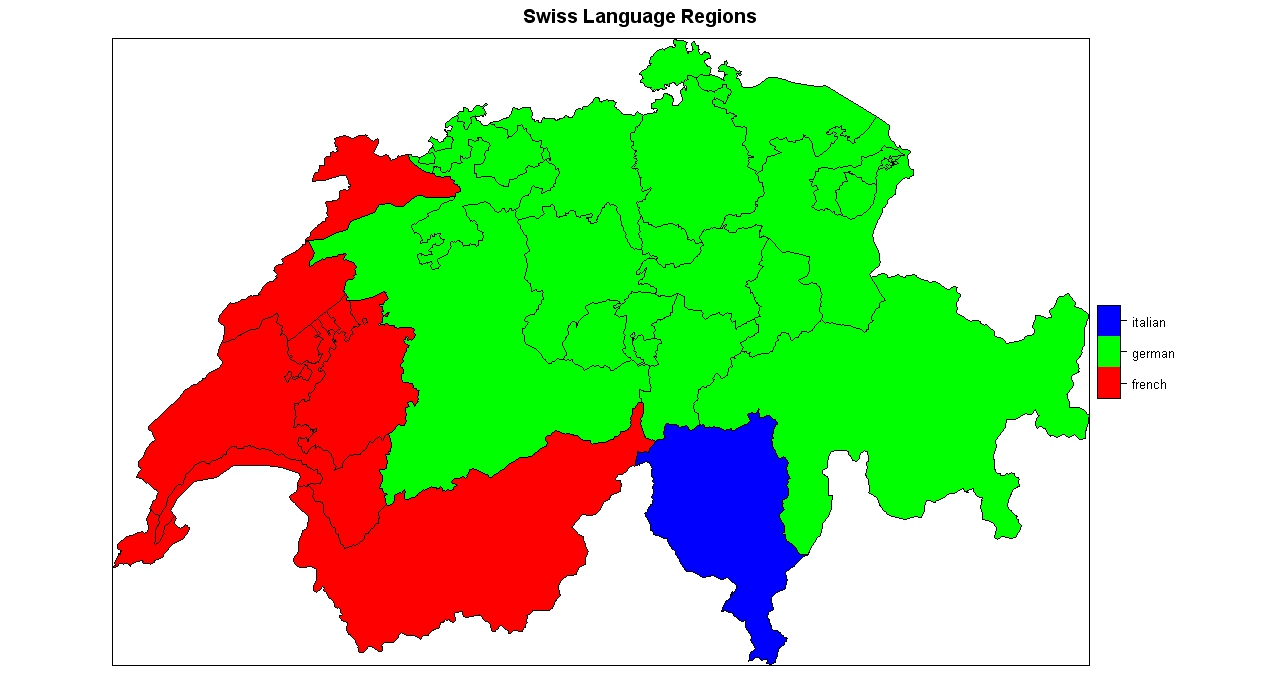
\includegraphics[width=0.96\linewidth]{./SwissLang}
\caption{}
\label{fig:SwissLang}
\end{figure}

\newpage
\subsection*{German Districts}
\begin{framed}
\begin{verbatim}
library(sp)
library(RColorBrewer)

# get spatial data for Germany on county level
con <- url("http://gadm.org/data/rda/DEU_adm3.RData")
print(load(con))
close(con)
# plot Germany with random colors
col = rainbow(length(levels(gadm$NAME_3)))
spplot(gadm, "NAME_3", col.regions=col, main="German Regions",
       colorkey = FALSE, lwd=.4, col="white")
\end{verbatim}
\end{framed}       

\begin{figure}
\centering
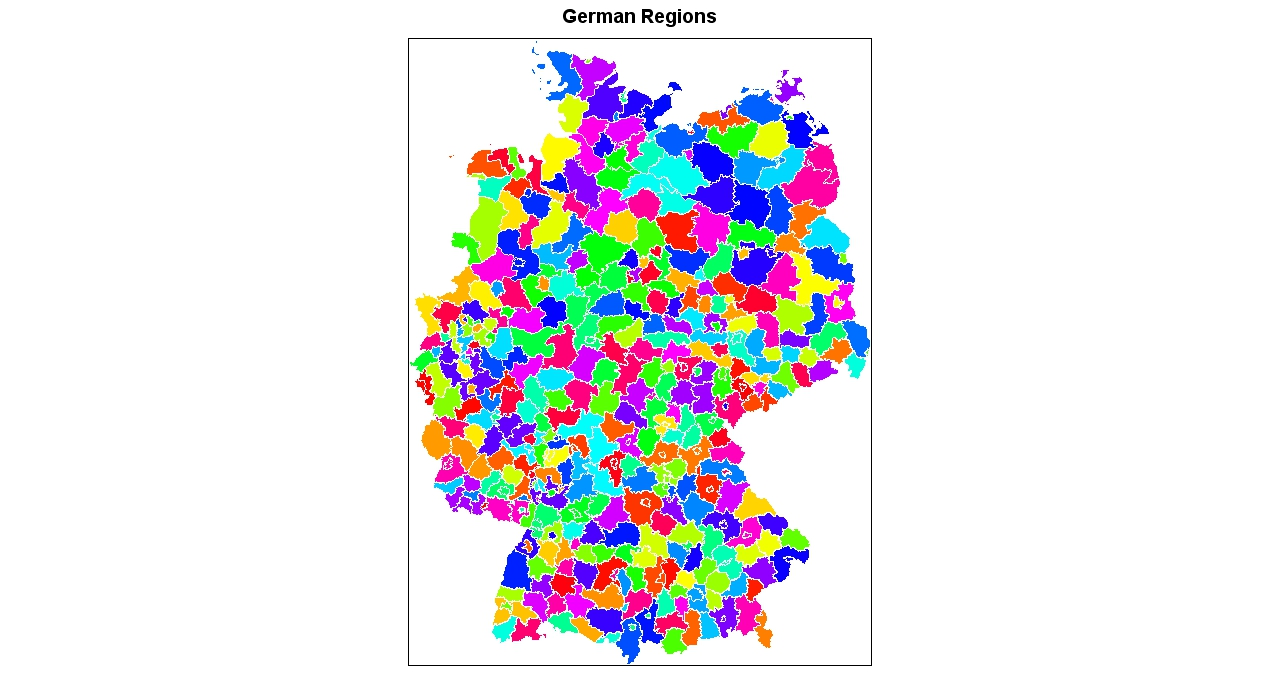
\includegraphics[width=0.96\linewidth]{./Germany}
\caption{}
\label{fig:Germany}
\end{figure}

\end{document}

